\documentclass[a4paper,10pt]{article}
\usepackage[utf8]{inputenc}
\usepackage{xspace}
\usepackage{graphicx,graphics} 
\usepackage{color}
\usepackage{amsmath}
\usepackage{amsfonts}
\usepackage{amssymb}
\usepackage{amsthm}
\usepackage{algorithm}
\usepackage{algorithmic}
\usepackage{longtable}
\usepackage{complexity}
\usepackage{tkz-graph}
\usepackage{float}
\usepackage{setspace}
\renewcommand{\algorithmicrequire}{\textbf{Input:}}
\renewcommand{\algorithmicensure}{\textbf{Output:}}
  
\graphicspath{{figures/}}
\newcommand\rmatching{${\cal R}$-matching\xspace}
\newcommand\mdelay{$\cal M$-delay\xspace}
\newcommand\matchedgraph{{\bf matched graph}}
\newtheorem{proposition}{Proposition}
\newtheorem{theorem}{Theorem}
\newcommand{\reporttitle}{Contention management for Deterministic Networking}     % Titre
\newcommand{\reportauthor}{Maël \textsc{Guiraud }} % Auteur
\newcommand{\reportsubject}{Master Thesis} 
\newcommand{\HRule}{\rule{\linewidth}{0.5mm}}
\setlength{\parskip}{1ex} % Espace entre les paragraphes


\newcommand{\todo}[1]{{\color{red} TODO: {#1}}}


%opening
\title{Contention Management for 5G}
\author{DB,CC,MG,OM,YS}


\begin{document}

\maketitle

\begin{abstract}
This article treats about Contention Management for 5G.
\end{abstract}

\section{Introduction}
  \itemize
    \item Context and problematic
    \item Related works
    \item Article contribution

\section{Model, Problems}

  \subsection{Definitions}
  
	We consider a symmetric directed graph $G=(V,A)$ modeling a slotted network. Each arc  $(u,v)$ in $A$ is characterized by an integer delay $Dl(u,v) \geq 1$ representing the number of slots from $u$ to $v$ on this arc. Note that for any arc $(u,v)$, $Dl(u,v)=Dl(v,u)$.

      A route $r$ in $G$ is a sequence of consecutive arcs $a_0, \ldots , a_{k-1}$, with $a_i=(u_i,u_{i+1}) \in A$.  The {\em latency} of a vertex $u_i$ in $r$, with $i \geq 1$, is defined by $$\lambda(u_i,r)= \sum\limits_{0 \leq j <i} Dl(a_j)$$ We also define $\lambda(u_0,r)=0$.
      The latency of the route $r$ is defined by $\lambda (r)= \lambda (u_k,r)$.  A routing function $\cal R$ in $G$ associates a route from $u$ to $v$ for any couple of different vertices $<u,v>$ in $G$.\\

      Let $\cal C$ be an {assignment} in $G$, i.e., set of couples of different vertices of $G$. We denote by $\cal R_{\cal C}$ the set of routes ${\cal R}(u,v)$ for any $<u,v>$ in $\cal C$. 

   \subsection{Slotted time Model}
      Consider now a positive integer $P$ called {\bf period}. A {\bf $P$-periodic affectation} of $\cal C$ in $(G,{\cal R})$ consists in a set  ${\cal M}=(m_0, \ldots ,m_{c-1})$
      of $c$ integers that we call {\bf offset}, with $c$ the cardinal of $\cal C$. Indeed, time is consider as consecutive periods of $P$ slots each and the number $m_i$ represents the first slot number used by the route $r_i \in {\cal R}_{\cal C}$ at its source.
      We define the first time slot at which a message reaches any vertex $v$ in this route by $$t(v,r_i) = m_i+\lambda(v,r_i) \mod P.$$

      Let us call $[t(v,r_i)]$ the values of the time slots used by a route $r_i$ in such a vertex $v$. 
      Those values are forming a continuous set of values starting at $t(v,r_i) \mod P$ and ending at $t(v,r_i) + \tau \mod P$. A $P$-periodic affectation must have no {\bf collision} between two routes in ${\cal R}_{\cal C}$, that is $\forall r_i, r_j \in {\cal R}_{\cal C}, i \ne j$, with $\tau$ the size (in number of consecutive slots) of each message that must be periodically sent on each route of ${\cal R}_{\cal C}$,
      we have $$[t(u,r_i)] \cap [t(u,r_j)] = \emptyset .$$
      
   \subsection{Problems}

      The main theoretical problem we have to deal with in this context is the following.\\

      \noindent {\bf Problem  Periodic Routes Assignment (PRA)} 

      \noindent {\bf Input:} graph $G=(V,A)$, set $\cal C$ of couples of vertices, routing function $\cal R$, integer $P$.

      \noindent {\bf Question:} does there exist a $P$-periodic affectation of $\cal C$ in $(G,{\cal R})$?

      We deal in next section with complexity of Problem PRA.\\

      \begin{figure}[H]
      \label{could-ran}
      \begin{center}
      % \begin{tabular}{cc}
      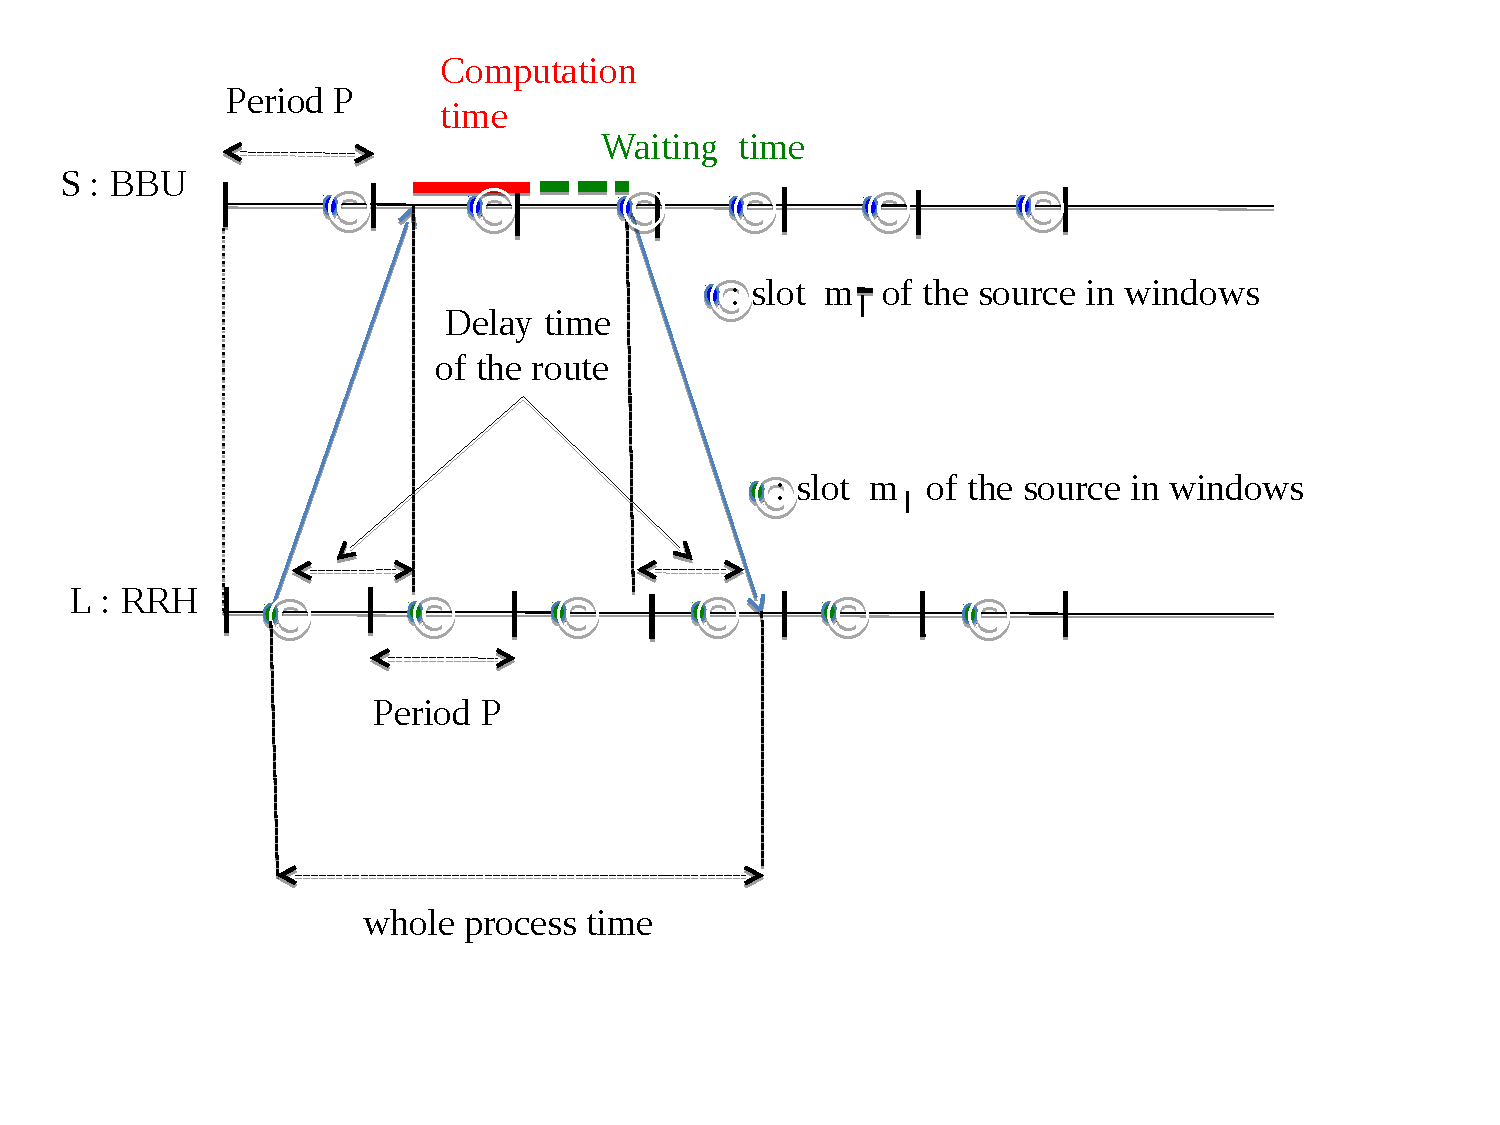
\includegraphics[scale=0.5]{Total-latence.pdf}
      \caption{Complete process for a leaf in $L$.}
      \end{center}
      \end{figure}
      %\end{tabular}\newline

      
      In the context of cloud-RAN applications, we consider here in digraph $G=(V,A)$ modeling the target network two disjoint subsets of vertices $S$ and $L$, where $S$ is the set of BBU and $L$ is the set of RRH. We consider a {\bf matching} defined as an application $\rho:S\rightarrow L$. We consider a $P$-periodic affectation $\cal M$, associating respectively integers $m_l$ and $m_{\overline l}$ to couples $(l,\rho(l))$ and $(\rho(l),l)$ for all $l \in L$. The process realized periodically (i.e. initiated in each window of size $P$) for each leaf $l \in L$ is the following one (see Figure \ref{cloud-ran}). First, a message of $\tau$ slots is sent from $l$ to $\rho(l)$ on ${\cal R}(l,\rho(l))$ at slot $m_l$ in the current window. After receiving this message, $\rho(l)$ computes it during a time equal to $\theta$ slots. Then, a message of $\tau$ slots containing the computed result is sent back from $\rho(l)$ to $l$ on ${\cal R}(\rho(l),l)$, at the first occurrence of  step $m_{\overline l}$ in a window (i.e., in the current window at the end of computation or the next one). We denote by $\omega(l)$ the {\bf waiting time}of $l$, i.e.,  the number of slots between the end of the computation time in $\rho(l)$ and the first occurrence of  step $m_{\overline l}$ in a window. Thus, the whole proccess time for $l$ is equal to
      $$
      PT(l)=\lambda({\cal R}(l,\rho(l)))+\theta+\omega(l)+\lambda({\cal R}(\rho(l),l)).
      $$
	
      Let us denote by ${\cal C}_{\rho}$ the set of couples $<l,\rho(l)>$ and $<\rho(l),l>$, for any $l \in L$. Consider a $P$-periodic affectation ${\cal M}$ of ${\cal C}_{\rho}$ in $(G,{\cal R})$. The maximum process time of ${\cal M}$ is equal to equal to $MT({\cal M})=\max\limits_{l \in L} PT(l)$. Thus, we have to deal with the following problem.\\

      \noindent {\bf Problem Periodic Assignment for Low Latency(PALL)} 

      \noindent {\bf Input:}  a digraph $G$, a matching $\rho$ of a set $S$ into a set $L$ in $G$, a routing function $\cal R$, a period $P$, an integer $T_{max}$.

      \noindent {\bf Question:} does there exist  a $P$-periodic affectation ${\cal M}$ of ${\cal C}_{\rho}$ in $(G,{\cal R})$ such that $MT({\cal M}) \leq T_{max}$?

      The related optimisation problem we will focus on  consists in minimizing  $MT({\cal M})$. Note that in the context of cloud-RAN networks, we consider $P=1ms$, $\theta=2.6ms$ and $T_{max}$ must be less or equal to $3ms$.


	

  
\section{PRA Solving}
  
  \subsection{NP-Hardness}
	
   
    \begin{theorem}
    Problem PRA cannot be approximate within a factor $n^{1-o(1)}$ unless $\P = \NP$ even when the load is two
    and $n$ is the number of vertices.
    \end{theorem}

    \begin{proof}
    We reduce PRA to graph coloring. Let $G$ be a graph instance of the $k$-coloring problem. 
    We define $H$ in the following way: for each vertex $v$ in $G$, there is a route $r_v$ in $H$.
    Two routes $r_v$ and $r_u$ share an edge if and only if $(u,v)$ is an edge in $G$ and this edge is only in this two routes. 
    We put weight inbetween shared edges in a route so that there is a delay $k$ between two such edges. 
    
    As in the previous proof, a $k$-coloring of $G$ gives a $k$-periodic schedule of $H$
    and conversly. Therefore if we can approximate the value of PRA  within a factor $f$,
    we could approximate the minimal number of colors needed to color a graph within a fator $f$, 
    by doing the previous reduction for all possible $k$. The proof follows from the hardness of approximability
    of finding a minimal coloring~\cite{zuckerman2006linear}.
    \end{proof}


   
  \subsection{MIN-PRA}
    Exemple de cas simple
    
\section{Proposed Solutions, solving PALL}

  \subsection{Intro}
    PALL NP-Hard car PRA NP-Hard\\
    Résultats valables sur Topologie 1 avec nos paramètres
    
  \subsection{No waiting times}
    \subsubsection{Star affectation}
      Définir star affectation en partant de PALL
    \subsubsection{Shortest-longest}
      \paragraph{Algo}
      \paragraph{Period}
    \subsubsection{Exhaustive generation}
      Décrire l'algo, expliquer les coupes
    \subsubsection{Results}
      Resultats des simulations : Shortest-longest optimal pour ces parametres.
      
   \subsection{Allowing waiting times}
     \subsubsection{Intro}
	Importance des waiting times quand la période est donnée (Résultats D'éxepriences et preuve avec l'exemple)
     \subsubsection{LSG}
	\paragraph{Algorithm}
	\paragraph{Analysis}
	  Parler de LSO et expliquer pourquoi LSG mieux avec nos params
     \subsubsection{Results}
	 \paragraph{Random}
	 \paragraph{Distributions}
   
\section{Conclusion}

\end{document}
